\section{Introduction}
{\setbeamertemplate{frame footer}{*\href{https://www.nature.com/subjects/conservation}{\textcolor{gray}{https://www.nature.com/subjects/conservation}}}
	\begin{frame}[t]{What is conservation biology?}
%	\begin{definition}<1->
Conservation biology is the study of attempts to protect and preserve \alert{biodiversity}*.
%	\end{definition}
%\begin{enumerate}[]
%	\item<2-> It focuses on:
%	\begin{itemize}		
%		\item<2-> both the biological and social factors that affect the success of conservation efforts
%		\item<2-> determining ecosystems and species whose conservation is a high priority
%	\end{itemize}
%	\item<3-> It has two central goals:
%	\begin{itemize}		
%		\item<3-> to evaluate human impacts on biodiversity
%		\item<3-> to develop practical approaches to prevent the extinction of species\cite{wilson1992diversity} (Soulé 1986, Wilson 1992)
%	\end{itemize}
%\end{enumerate}
\begin{block}<2->{It focuses on}
	\begin{itemize}		
		\item<2-> both the biological and social factors that affect the success of conservation efforts
		\item<2-> determining ecosystems and species whose conservation is a high priority
	\end{itemize}
\end{block}

\begin{block}<3->{It has two central goals}
	\begin{itemize}		
		\item<3-> to evaluate human impacts on biodiversity
		\item<3-> to develop practical approaches to prevent the extinction of species\cite{wilson1992diversity} (Soulé 1986, Wilson 1992)
	\end{itemize}
\end{block}

\end{frame}}

%below will be a frame with only one picture full creeen:
%\begin{frame}[plain]
%\makebox[\linewidth]{\parbox{\paperwidth}{\animategraphics[loop,autoplay,width=\paperwidth]{5}{amazon_deforestation-}{0}{12}}}
%\end{frame}

{\setbeamertemplate{frame footer}{*\href{https://www.nature.com/scitable/knowledge/library/conservation-of-biodiversity-13235087}{\textcolor{gray}{https://www.nature.com/scitable/knowledge/library/conservation-of-biodiversity-13235087}}}
	\begin{frame}[t]{We are losing biodiversity}
	\begin{itemize}
		\item Modern extinction rates are at \alert{100} to \alert{1000} times greater than background extinction rates calculated over the eras \cite{hambler2004extinction}
		\item Existing species go extinct at a rate \alert{1000} times that of species formation*
		\item The primary cause of today's loss of biodiversity is \alert{habitat alteration caused by human activities}
	\end{itemize}	
\end{frame}
}

{\setbeamertemplate{frame footer}{\href{https://earthobservatory.nasa.gov/world-of-change/Deforestation}{\textcolor{gray}{https://earthobservatory.nasa.gov/world-of-change/Deforestation}}}
	\begin{frame}{Deforestation in Amazon}
	\centering
	\animategraphics[loop,autoplay,width=\textwidth]{2}{amazon_deforestation-}{0}{12}
\end{frame}
}

\begin{frame}{Proportion of population using improved drinking water sources (\%), 1990}
\makebox[\linewidth]{\parbox{\paperwidth}{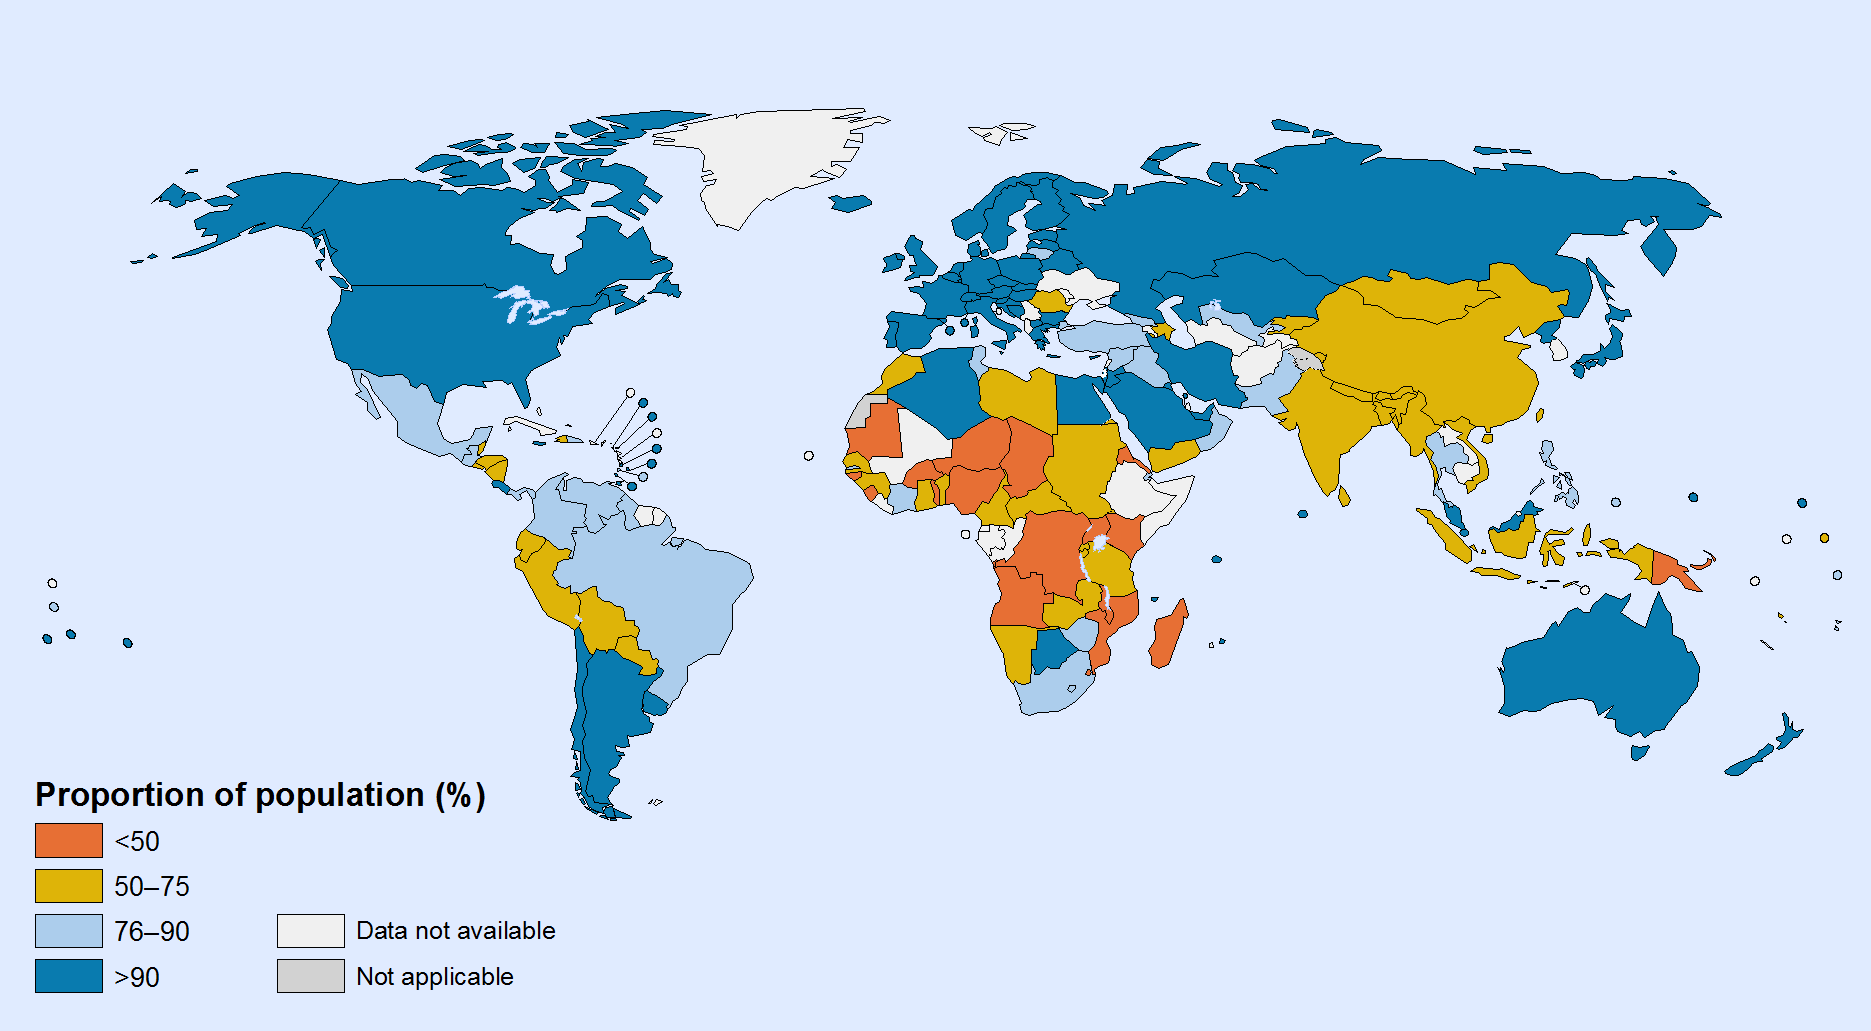
\includegraphics[width=\paperwidth]{Global_water_1990}}}
\end{frame}

\begin{frame}{Proportion of population using improved drinking water sources (\%), 2000}
\makebox[\linewidth]{\parbox{\paperwidth}{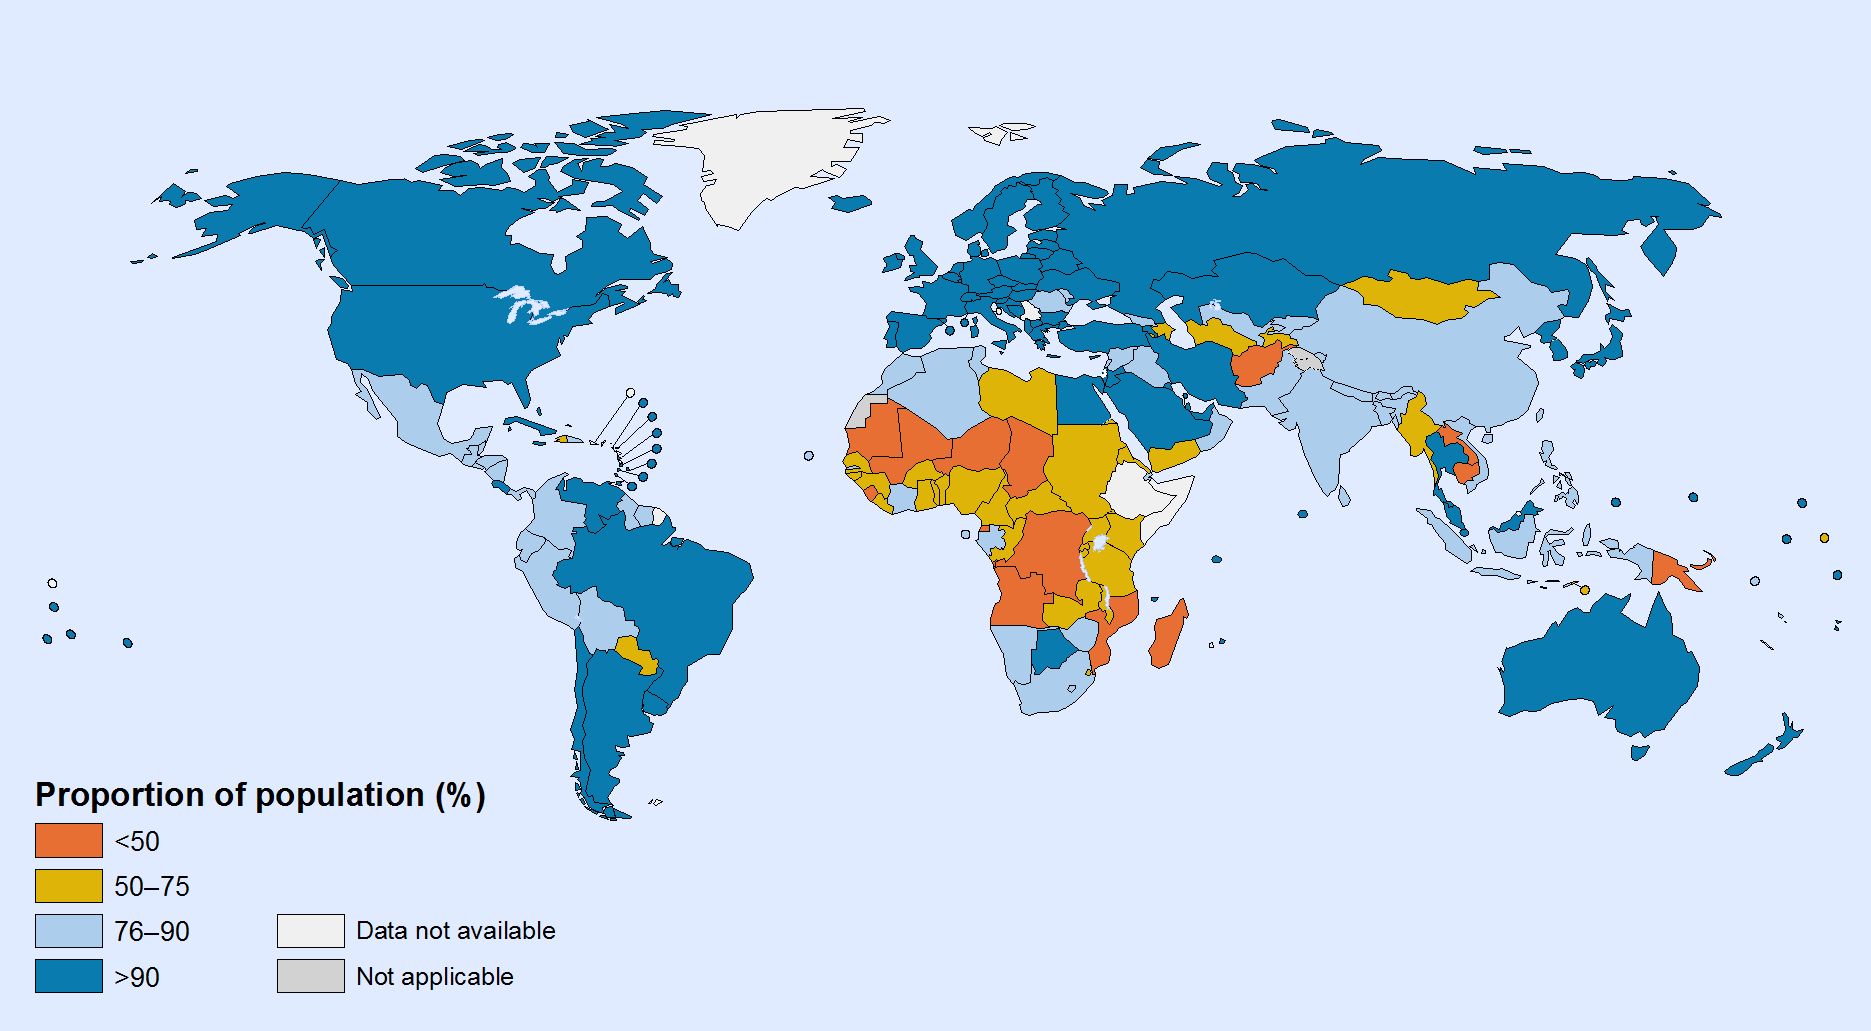
\includegraphics[width=\paperwidth]{Global_water_2000}}}
\end{frame}

\begin{frame}{Proportion of population using improved drinking water sources (\%), 2015}
\makebox[\linewidth]{\parbox{\paperwidth}{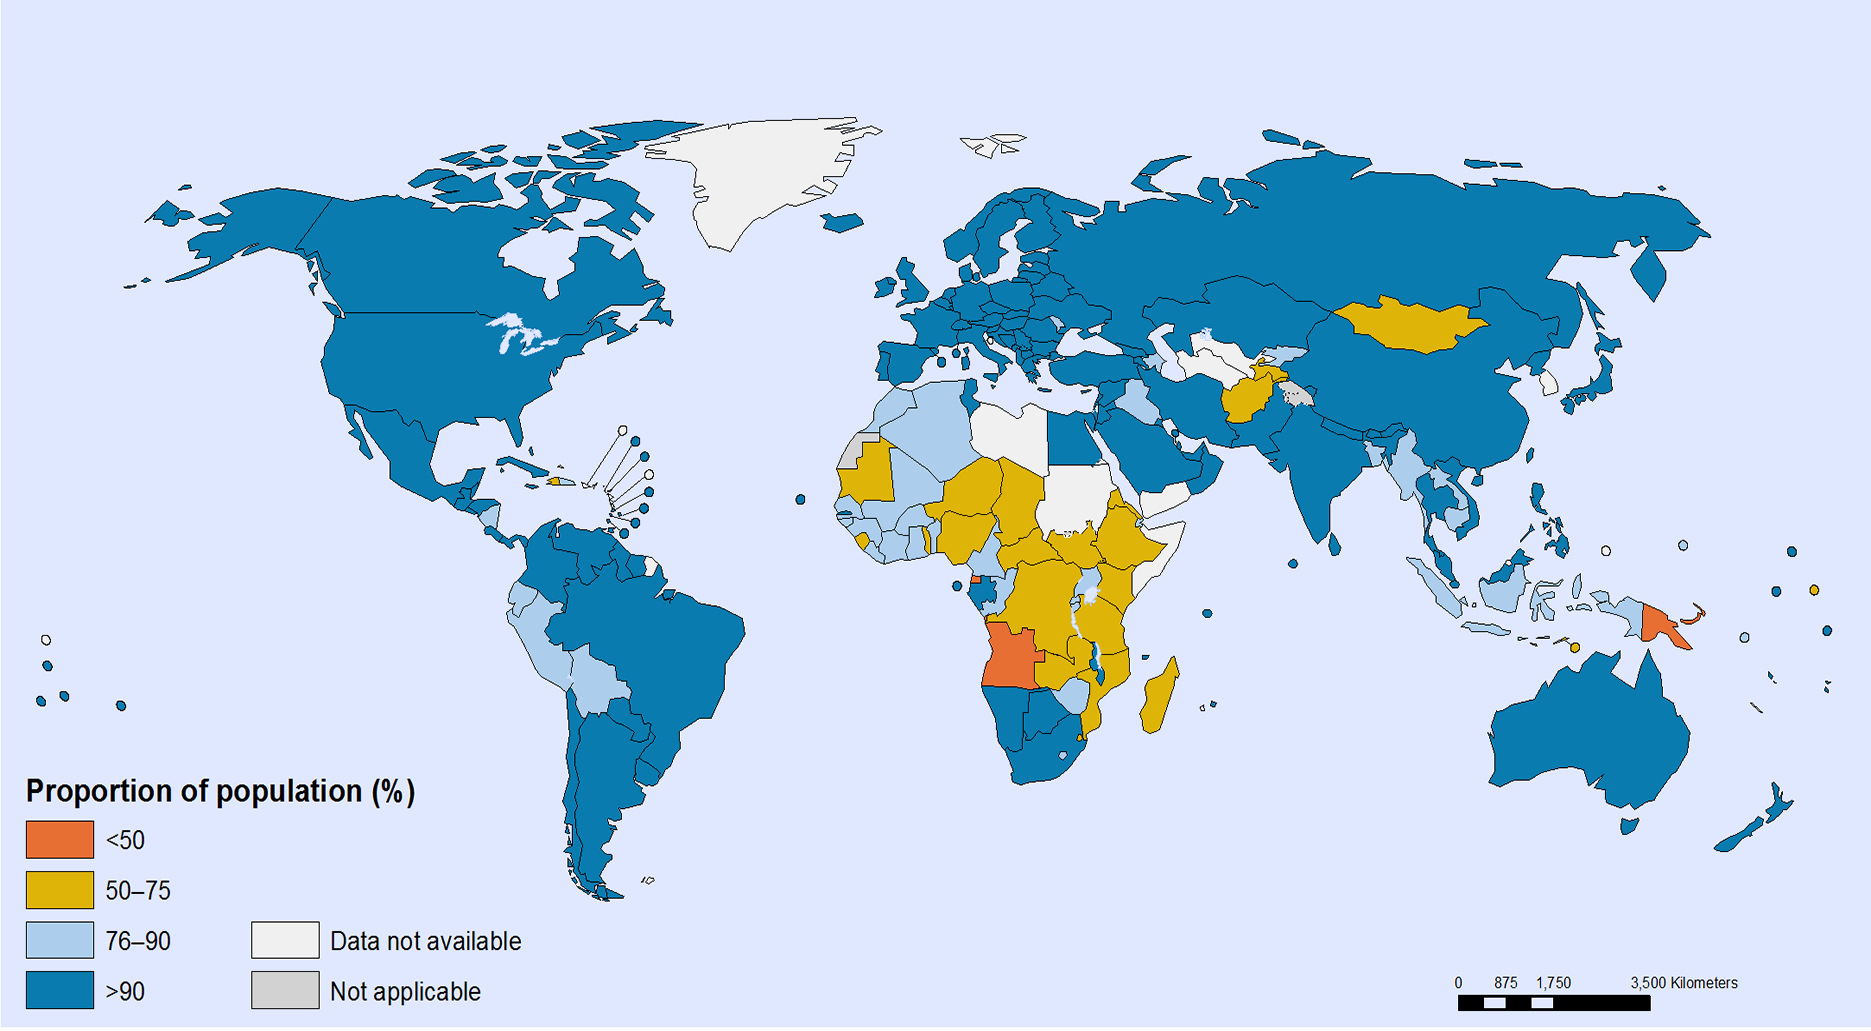
\includegraphics[width=\paperwidth]{Global_water_2015}}}
\end{frame}

\begin{frame}{Proportion of population using improved sanitation facilities (\%), 1990}
\makebox[\linewidth]{\parbox{\paperwidth}{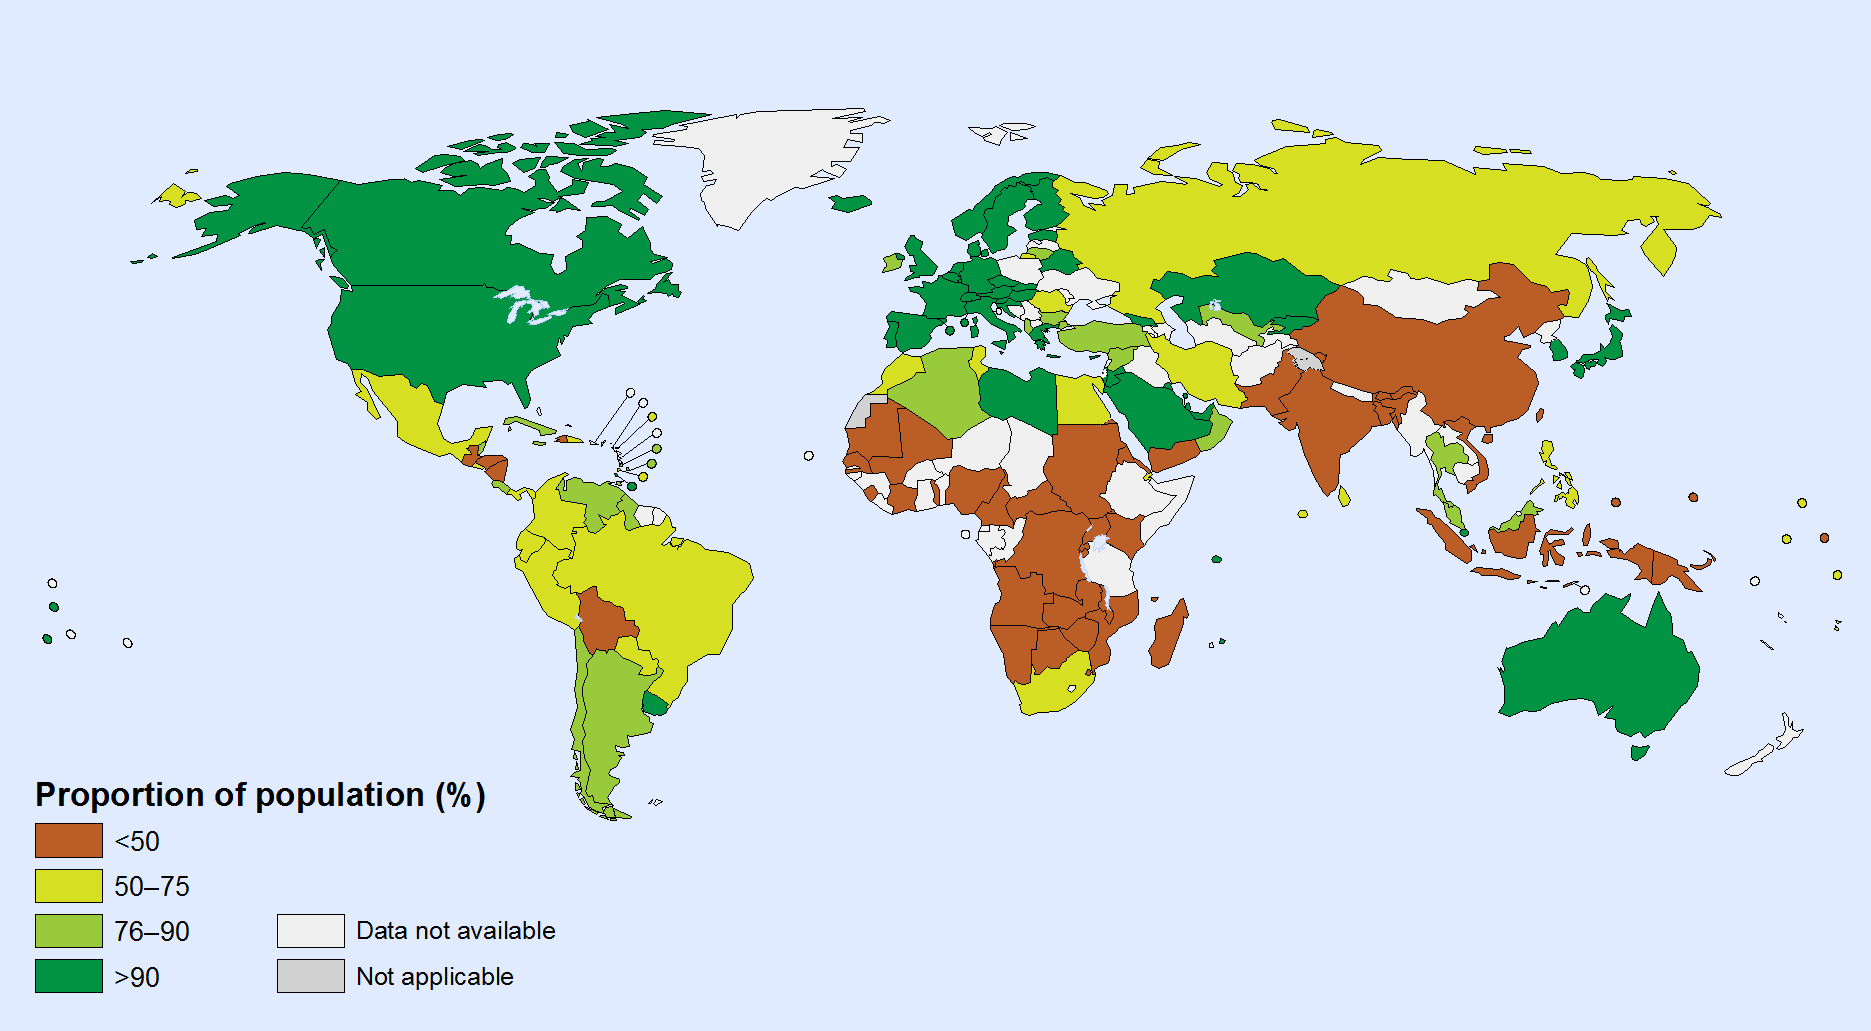
\includegraphics[width=\paperwidth]{Global_sanitation_1990}}}
\end{frame}

\begin{frame}{Proportion of population using improved sanitation facilities (\%), 2000}
\makebox[\linewidth]{\parbox{\paperwidth}{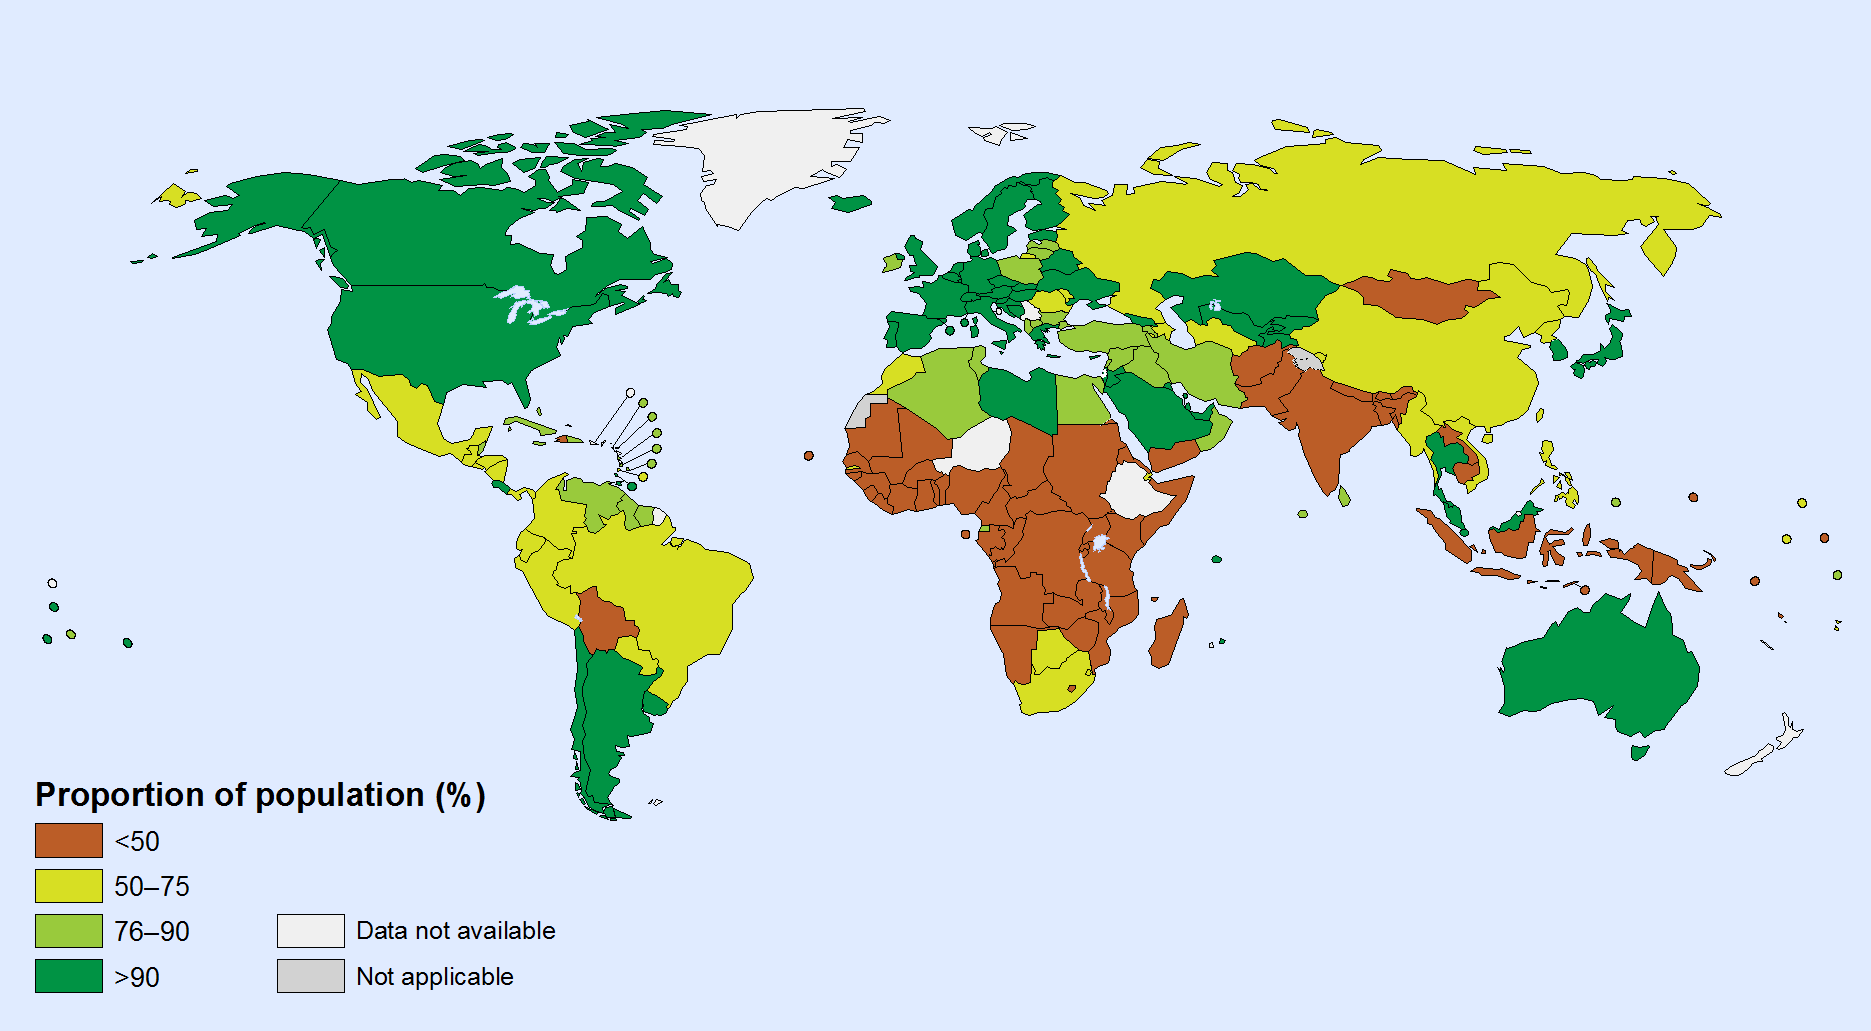
\includegraphics[width=\paperwidth]{Global_sanitation_2000}}}
\end{frame}

\begin{frame}{Proportion of population using improved sanitation facilities (\%), 2015}
\makebox[\linewidth]{\parbox{\paperwidth}{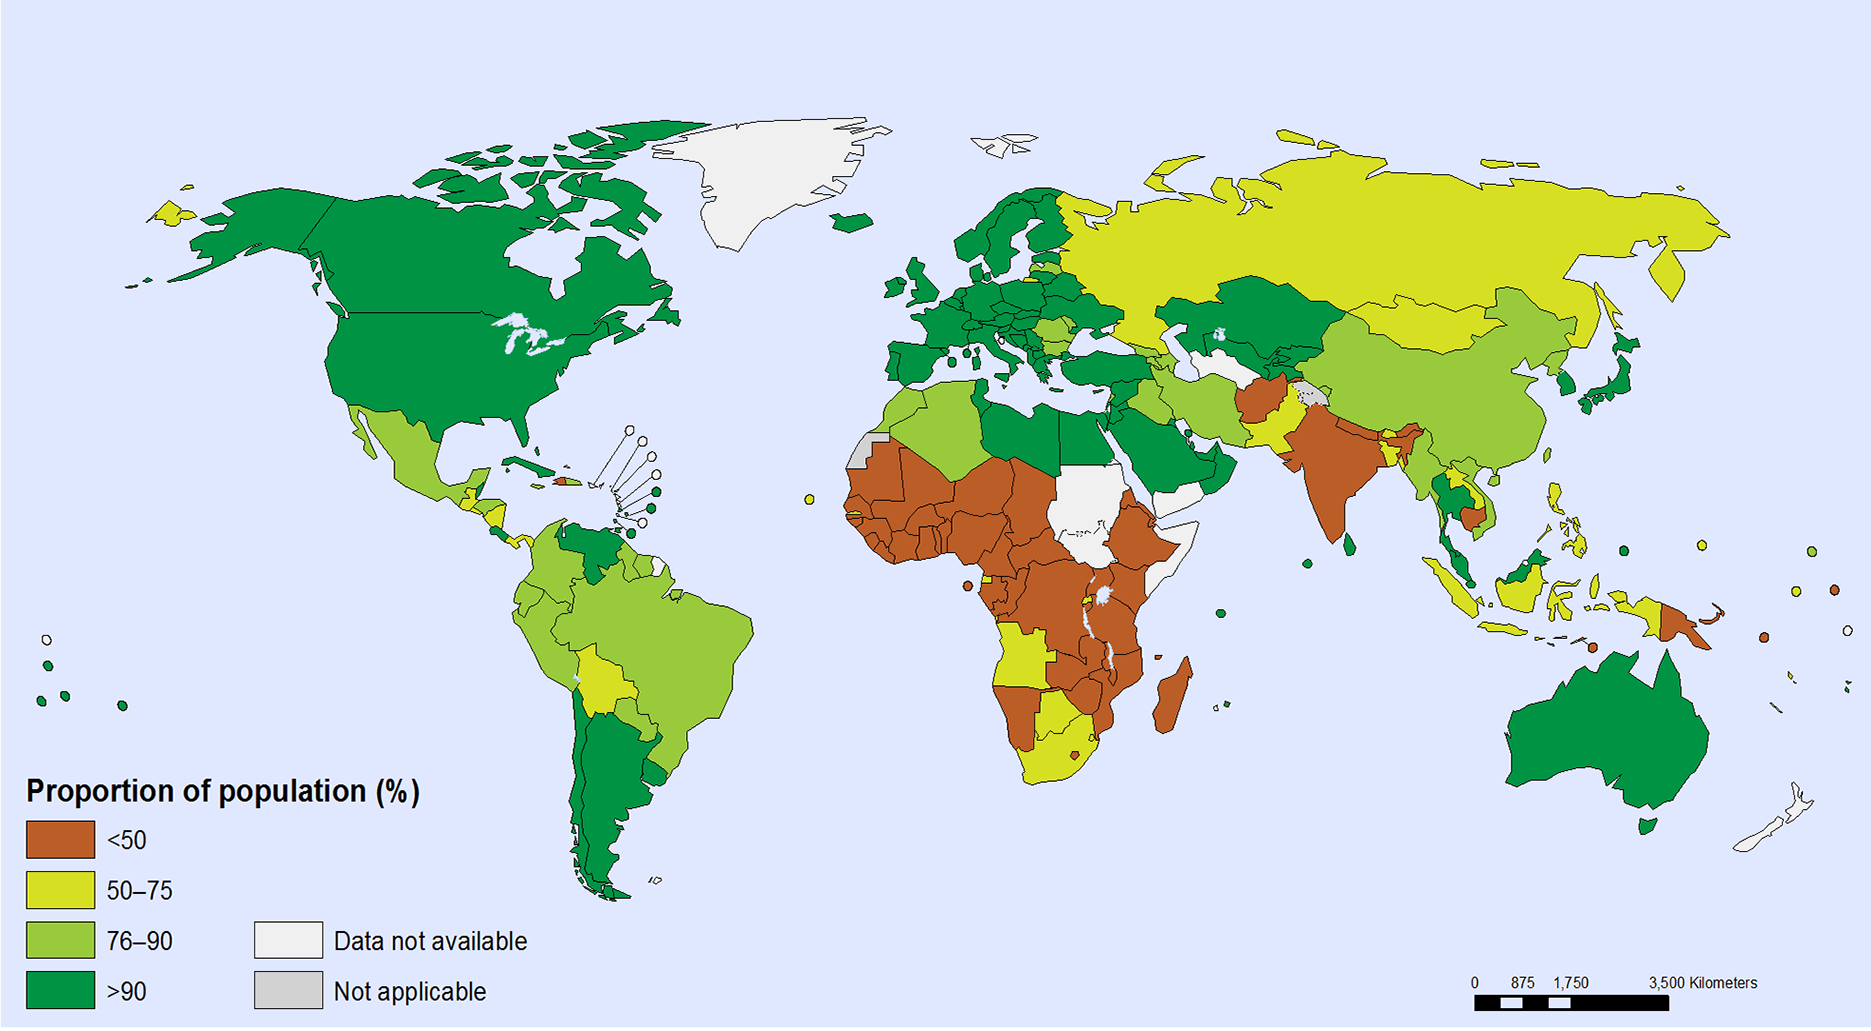
\includegraphics[width=\paperwidth]{Global_sanitation_2015}}}
\end{frame}

\begin{frame}{Surface water quality in China}
  \makebox[\linewidth]{\parbox{\paperwidth}{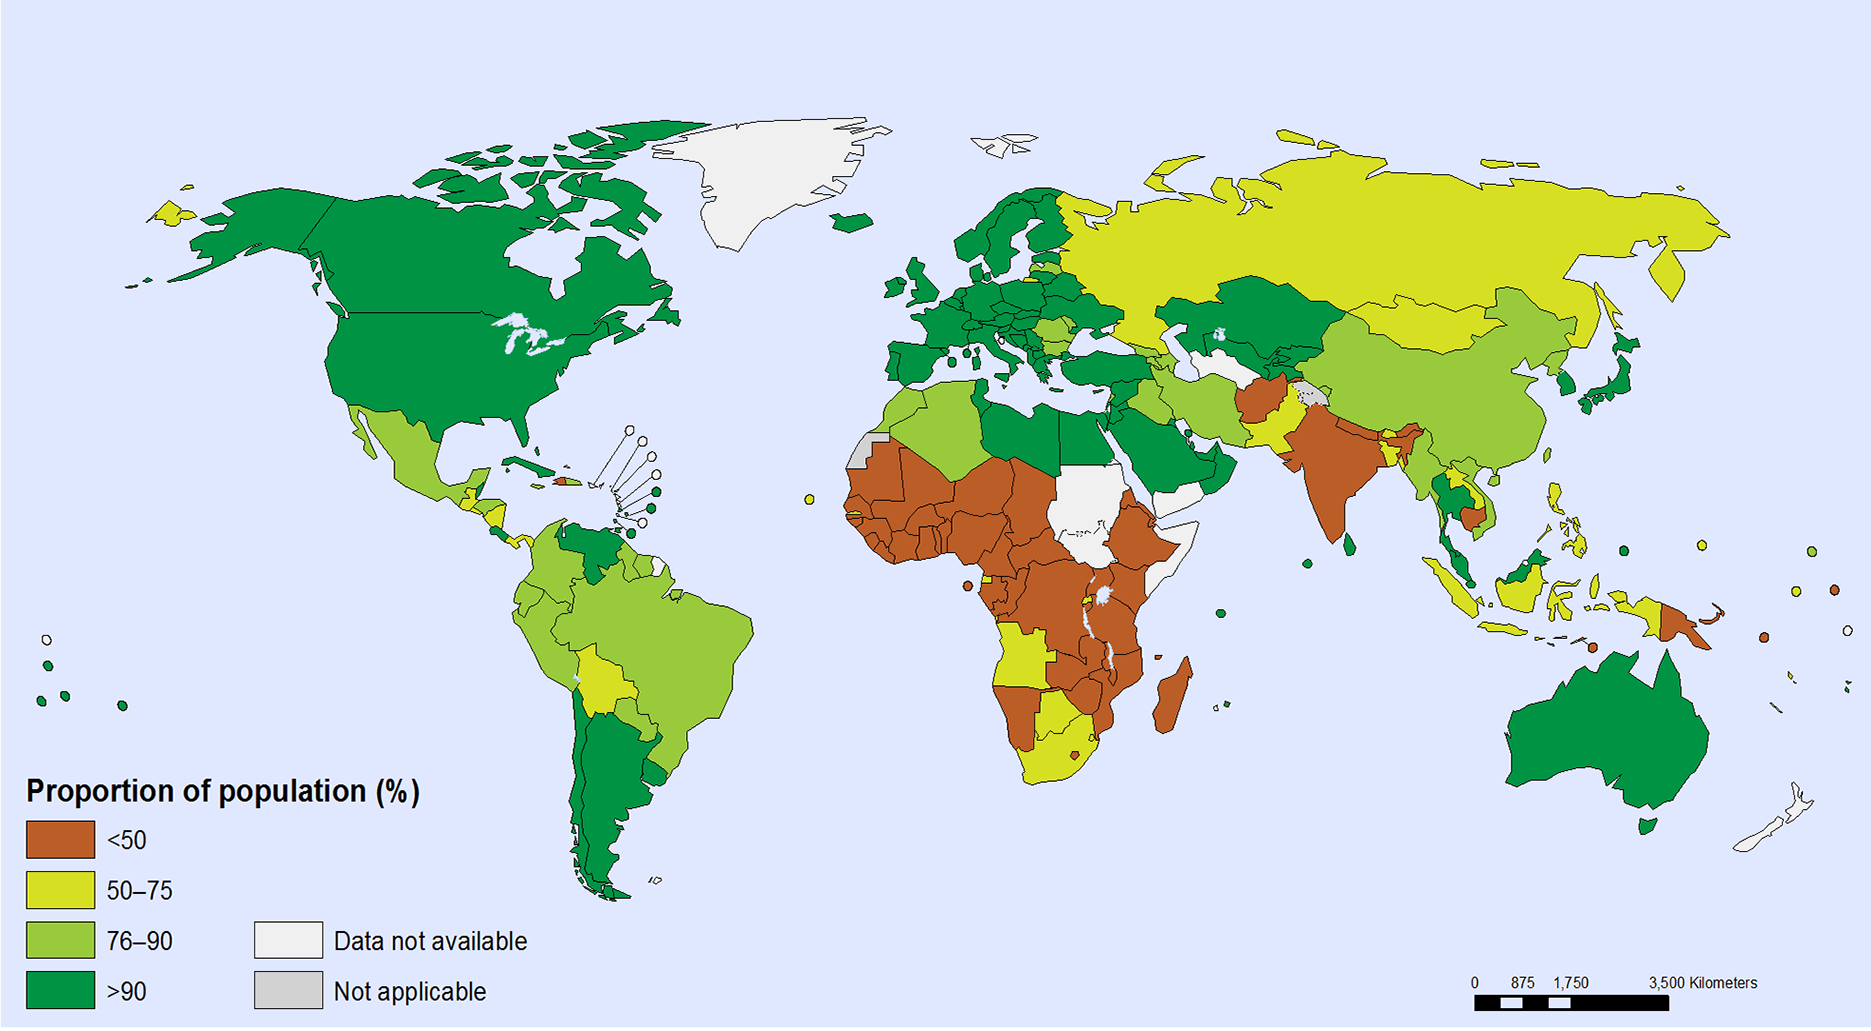
\includegraphics[width=\paperwidth]{Global_sanitation_2015}}}
\end{frame}

\begin{frame}{Water quanlity of China's lakes}
  \makebox[\linewidth]{\parbox{\paperwidth}{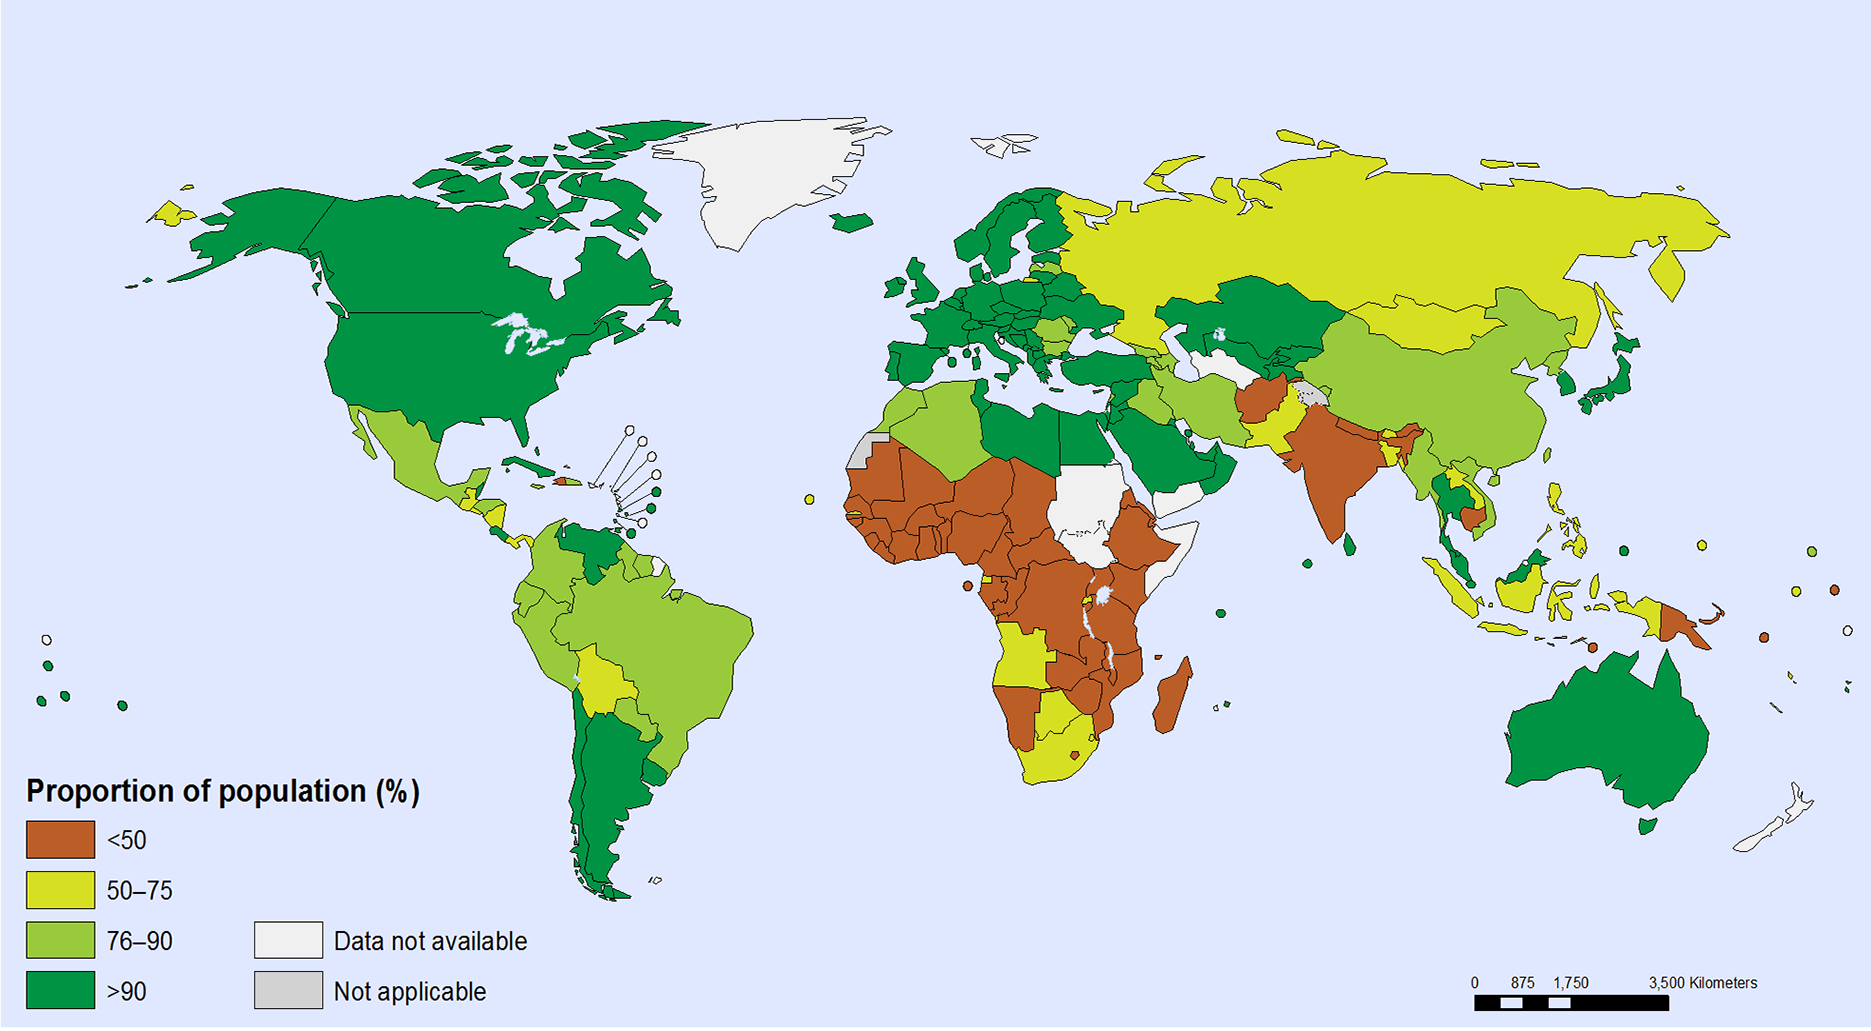
\includegraphics[width=\paperwidth]{Global_sanitation_2015}}}
\end{frame}
